
%----------------------------------------------------------------------------------------
%	PACKAGES AND OTHER DOCUMENT CONFIGURATIONS
%----------------------------------------------------------------------------------------

\documentclass[12pt]{article}

\usepackage{graphicx}
\usepackage{epsfig}
\usepackage{psfrag}
%\usepackage{subfigure}
%\usepackage{subfig}
%\usepackage{tabularx}
\usepackage{subfigmat}
\usepackage{subeqnarray}
\usepackage[colorlinks]{hyperref}
\usepackage{amsmath,amsfonts,amsfonts,amsthm}
\usepackage{xcolor,colortbl}
\usepackage[mathscr]{euscript}
\usepackage{algorithm2e}
\usepackage{siunitx}
\usepackage{rotating}
\usepackage{bm}
\setcounter{secnumdepth}{3}
\usepackage[version=3]{mhchem} 
\usepackage{graphicx}
\usepackage{fancyvrb}
\usepackage[top=1in, bottom=1in, left=1in, right=1in]{geometry}
\graphicspath{{../Figures/}}
\usepackage{color}
\usepackage{pdfpages}
\usepackage{enumitem}
\usepackage{bbm}

\newcommand\alignedbox[2]{
	% Argument #1 = before & if there were no box (lhs)
	% Argument #2 = after & if there were no box (rhs)
	&  % Alignment sign of the line
	{
		\settowidth\dlf{$\displaystyle #1$}  
		% The width of \dlf is the width of the lhs, with a displaystyle font
		\addtolength\dlf{\fboxsep+\fboxrule}  
		% Add to it the distance to the box, and the width of the line of the box
		\hspace{-\dlf}  
		% Move everything dlf units to the left, so that & #1 #2 is aligned under #1 & #2
		\boxed{#1 #2}
		% Put a box around lhs and rhs
	}
}
%----------------------------------------------------------------------------------------
%	ABBREVIATIONS SECTIONS
%----------------------------------------------------------------------------------------
 \newcommand{\dod}{\mathrm{C}_{12}\mathrm{H}_{26}}
 \newcommand{\nit}{\mathrm{N}_{2}}
 \newcommand{\ox}{\mathrm{O}_{2}}
 \newcommand{\wat}{\mathrm{H}_{2}\mathrm{O}}
 \newcommand{\cardiox}{\mathrm{C}\mathrm{O}_{2}}

\begin{document}
%
%%%%%%%%%%%%%%%%%%%%%%%%%%%%%%%%%%%%%%%%%%%%%%%%%%%%%%%%%%%%%%%%%%%%%%
%
\makeatletter
\newcommand\rlarrows{\mathop{\operator@font \rightleftarrows}\nolimits}
\makeatother
%
%%%%%%%%%%%%%%%%%%%%%%%%%%%%%%%%%%%%%%%%%%%%%%%%%%%%%%%%%%%%%%%%%%%%%%
\newenvironment{itemizePacked}{
\begin{itemize}
  \setlength{\itemsep}{1pt}
  \setlength{\parskip}{0pt}
  \setlength{\parsep}{0pt}
}{\end{itemize}}
\newenvironment{enumeratePacked}{
\begin{enumerate}
  \setlength{\itemsep}{5pt}
  \setlength{\parskip}{0pt}
  \setlength{\parsep}{0pt}
}{\end{enumerate}}
% abbreviations %%%%%%%%%%%%%%%%%%%%%%%%%%%%%%%%%%%%%%%%%%%%%%%%%%%%%%
%
%\def\codefont{scriptsize}
\newcommand{\f}[2]{{\frac{#1}{#2}}}
\newcommand{\wt}[1]{{\widetilde{#1}}}
\newcommand{\wh}[1]{{\widehat{#1}}}
\newcommand{\wc}[1]{{\widecheck{#1}}}
\newcommand{\chem}[1]{\ensuremath{\mathrm{#1}}}
\newcommand{\lrangle}[1]{{\langle{#1}\rangle}}
\newcommand{\lrcurl}[1]{{\{{#1}\}}}
\newcommand{\ol}[1]{{\overline{#1}}}
%\newcommand{\ul}[1]{{\underline{#1}}}
\newcommand{\tr}{{\scriptscriptstyle\mathsf T}}
\newcommand{\dd}{{\scriptscriptstyle\Delta}}
\newcommand{\eps}{{\varepsilon}}

\def\RPP{reaction progress parameter}

% boldface-italic font
\newcommand{\bfit}[1]{\textbf{\textit{#1}}}

%
% SOME COLORS %%%%%%%%%%%%%%%%%%%%%%%%%%%%%%%%%%%%%%%%%%%%%%%%%%%%%%%%
%
\newcommand{\colred}[1]{{\color{red} #1}}
\newcommand{\colblue}[1]{{\color{blue} #1}}
\newcommand{\colwhite}[1]{{\color{white} #1}}
\newcommand{\colgreen}[1]{{\color{green} #1}}
\newcommand{\colbrown}[1]{{\color{Brown} #1}}
\newcommand{\colfucsia}[1]{{\color{Fuchsia} #1}}
\newcommand{\colBlue}[1]{{\color{Blue} #1}}
\newcommand{\corrections}[1]{{\color{blue}#1}}
\newcommand{\comment}[1]{{\color{blue}\bf{[#1]}}}
%
% FOR COMBUSTION TEXT %%%%%%%%%%%%%%%%%%%%%%%%%%%%%%%%%%%%%%%%%%%%%%%%
%
\def\chist{\chi_{Z,\up{st}}}
\def\chiq{\chi_{Z,\up{q}}}
\def\chii{\chi_{Z,\up{i}}}
%
% Standard TEX-abbreviations used %%%%%%%%%%%%%%%%%%%%%%%%%%%%%%%%%%%%
%
\def\cldbpage{\clearpage{\pagestyle{empty}\cleardoublepage}}
%
% CALIGRAPHICAL SYMBOLS %%%%%%%%%%%%%%%%%%%%%%%%%%%%%%%%%%%%%%%%%%%%%%
%
\def\cA{{\cal{A}}}
\def\cB{{\cal{B}}}
\def\cC{{\cal{C}}}
\def\cO{{\cal{O}}}
\def\cD{{\cal{D}}}
\def\cE{{\cal{E}}}
\def\cF{{\cal{F}}}
\def\cH{{\cal{H}}}
\def\cJ{{\cal{J}}}
\def\cG{{\cal{G}}}
\def\cN{{\cal{N}}}
\def\cL{{\cal{L}}}
\def\cS{{\cal{S}}}
\def\cT{{\cal{T}}}
\def\cU{{\cal{U}}}
\def\cC{{\cal{C}}} 
\def\cZ{{\cal{Z}}}
\def\cM{{\cal{M}}}
\def\cP{{\cal{P}}}
\def\cR{{\cal{R}}}
\def\cV{{\cal{V}}}
\def\cQ{{\cal{Q}}}
%
% NEW FUNCTION NAMES %%%%%%%%%%%%%%%%%%%%%%%%%%%%%%%%%%%%%%%%%%%%%%%%%
%
\def\erf{{\rm{erf}}}
%
% TEXT FONT DEFINITIONS %%%%%%%%%%%%%%%%%%%%%%%%%%%%%%%%%%%%%%%%%%%%%%
%
\def\up{\textup}
\def\p{\partial}
\def\d{\textup d}
\def\D{\displaystyle}
%\def\S{\scriptsize}
\def\OmFint{\iiint\limits_{\OmF}}
\def\OmF{{\Omega_{\cal F}}}
\def\OmA{{\Omega_{\cal A}}}
\def\e{\textup{e}}
\def\i{\textup{i}}
\def\REFUP{\rm{ref}}
\def\REF{_{\REFUP}}
%
% DIMENSIONLESS QUANTITIES %%%%%%%%%%%%%%%%%%%%%%%%%%%%%%%%%%%%%%%%%%%
%
%\def\Re{{\rm{Re}}}
\def\Fr{{\rm{Fr}}}
\def\M{{\rm{M}}}
\def\Ce{{\rm{Ce}}}
\def\Re{{\rm{Re}}}
\def\Rd{{\rm{Rd}}}
\def\Le{{\rm{Le}}}
\def\Da{{\rm{Da}}}
\def\Ka{{\rm{Ka}}}
\def\Nu{{\rm{Nu}}}
\def\Sc{{\rm{Sc}}}
\def\Ri{{\rm{Ri}}}
\def\Ec{{\rm{Ec}}}
\def\Tu{{\rm{Tu}}}
\def\St{{\rm{St}}}
\def\Mi{{\rm{Mi}}}
\def\Ra{{\rm{Ra}}}
\def\Ze{{\rm{Ze}}}
%
% FOR LATEX %%%%%%%%%%%%%%%%%%%%%%%%%%%%%%%%%%%%%%%%%%%%%%%%%%%%%%%%%%
%
 \def\avec{{\mbox{\boldmath$a$}}}
 \def\bvec{{\mbox{\boldmath$b$}}}
 \def\Bvec{{\mbox{\boldmath$B$}}}
 \def\cvec{{\mbox{\boldmath$c$}}}
 \def\dvec{{\mbox{\boldmath$d$}}}
 \def\evec{{\mbox{\boldmath$e$}}}
 \def\Fvec{{\mbox{\boldmath$F$}}}
 \def\Nvec{{\mbox{\boldmath$N$}}}
 \def\fvec{{\mbox{\boldmath$f$}}}
 \def\gvec{{\mbox{\boldmath$g$}}}
 \def\hvec{{\mbox{\boldmath$h$}}}
 \def\ivec{{\mbox{\boldmath$i$}}}
 \def\jvec{{\mbox{\boldmath$j$}}}
 \def\kvec{{\mbox{\boldmath$k$}}}
 \def\pvec{{\mbox{\boldmath$p$}}}
 \def\Pvec{{\mbox{\boldmath$P$}}}
 \def\uvec{{\mbox{\boldmath$u$}}}
 \def\Uvec{{\mbox{\boldmath$U$}}}
 \def\nvec{{\mbox{\boldmath$n$}}}
 \def\tvec{{\mbox{\boldmath$t$}}}
 \def\Rvec{{\mbox{\boldmath$R$}}}
 \def\rvec{{\mbox{\boldmath$r$}}}
 \def\svec{{\mbox{\boldmath$s$}}}
 \def\Svec{{\mbox{\boldmath$S$}}}
 \def\xvec{{\mbox{\boldmath$x$}}}
 \def\vvec{{\mbox{\boldmath$v$}}}
 \def\wvec{{\mbox{\boldmath$w$}}}
 \def\yvec{{\mbox{\boldmath$y$}}}
 \def\mvec{{\mbox{\boldmath$m$}}}
 \def\Xvec{{\mbox{\boldmath$X$}}}
 \def\qvec{{\mbox{\boldmath$q$}}}
 \def\0vec{{\mbox{\boldmath$0$}}}
 \def\xivec{{\mbox{\boldmath$\xi$}}}
 \def\rhovec{{\mbox{\boldmath$\rho$}}}
 \def\wpvec{{\boldsymbol{\wp}}}
 \def\psivec{{\mbox{\boldmath$\psi$}}}
 \def\epsvec{{\mbox{\boldmath$\epsilon$}}}
 \def\phivec{{\mbox{\boldmath$\phi$}}}
 \def\varphivec{{\mbox{\boldmath$\varphi$}}}
 \def\zetavec{{\mbox{\boldmath$\zeta$}}}
 \def\kappavec{{\mbox{\boldmath$\kappa$}}}
 \def\varkappavec{{\pmb{\varkappa}}}
 \def\etavec{{\mbox{\boldmath$\eta$}}}
 \def\Psivec{{\boldsymbol{\Psi}}}
 \def\Phivec{{\boldsymbol{\Phi}}}
 \def\Wvec{{\boldsymbol{W}}}
 \def\Yvec{{\mbox{\boldmath$Y$}}}
 \def\Vvec{{\mbox{\boldmath$V$}}}
 \def\cLvec{{\boldsymbol{\cal{L}}}}
 \def\cMvec{{\boldsymbol{\cal{M}}}}
 \def\omegavec{{\mbox{\boldmath$\omega$}}}
 \def\Omegavec{{\mbox{\boldmath$\Omega$}}}
 \def\sigmavec{{\boldsymbol{\sigma}}}
 \def\Amat{{\underline{\underline{{A}}}}}
 \def\Bmat{{\underline{\underline{{B}}}}}
 \def\Phimat{{\underline{\underline{{\Phi}}}}}
 \def\taumat{{\underline{\underline{{\tau}}}}}
 \def\sigmamat{{\underline{\underline{{\sigma}}}}}
 \def\Cmat{{\underline{\underline{{C}}}}}
 \def\Imat{{\underline{\underline{{I}}}}}
 \def\Jmat{{\underline{\underline{{J}}}}}
 \def\Smat{{\underline{\underline{{S}}}}}
 \def\Rmat{{\underline{\underline{{R}}}}}
 \def\Tmat{{\underline{\underline{{T}}}}}
 \def\Emat{{\underline{\underline{{E}}}}}
 \def\tmat{{\underline{\underline{{t}}}}}

 \def\alphavec{{\boldsymbol{\alpha}}}
 \def\betavec{{\boldsymbol{\beta}}}
 \def\tauvec{{\boldsymbol{\tau}}}
 \def\thetavec{{\boldsymbol{\theta}}}
 \def\lambdavec{{\mbox{\boldmath$\lambda$}}}
 \def\cTmat{{\underline{\underline{{\cal{T}}}}}}
 \def\cLmat{{\underline{\underline{{\cal{L}}}}}}
 \def\cMmat{{\underline{\underline{{\cal{M}}}}}}
 \def\kappamat{{\underline{\underline{{\kappa}}}}}
%
% Grad, Div, ... %%%%%%%%%%%%%%%%%%%%%%%%%%%%%%%%%%%%%%%%%%%%%%%%%%%%%
%
\def\Grad{\nabla}
\def\Div{\nabla \cdot}
\def\Lap{\nabla^2}
%

\begin{titlepage}

\newcommand{\ddz}[1]{\frac{\mathrm{d} #1}{\mathrm{d} z}}
\newcommand{\HRule}{\rule{\linewidth}{0.5mm}} % Defines a new command for the horizontal lines, change thickness here

\center % Center everything on the page
 

 
%----------------------------------------------------------------------------------------
%	HEADING SECTIONS
%----------------------------------------------------------------------------------------


%\textsc{\Large STANFORD UNIVERSITY}\\[1.5cm] % Name of your university/college

%----------------------------------------------------------------------------------------
%	TITLE SECTION
%----------------------------------------------------------------------------------------

\HRule \\[1 cm]
{ \huge \bfseries Problem Set 4 Solutions}\\[0.4cm] % Title of your document
\HRule \\[2cm]
 
%----------------------------------------------------------------------------------------
%	AUTHOR SECTION
%----------------------------------------------------------------------------------------

\Large  \textsc{Matthias Ihme}\\[2cm] % Your name
\textsc{\large ME 257/357: Propulsion System and Gas-Turbine Analysis}\\[2cm] % Major heading such as course name

%----------------------------------------------------------------------------------------
%	LOGO SECTION
%----------------------------------------------------------------------------------------

\includegraphics[width=50mm]{stanford_seal.png}\\[2cm] % Include a department/university logo - this will require the graphicx package
%----------------------------------------------------------------------------------------
%----------------------------------------------------------------------------------------
%	DATE SECTION
%----------------------------------------------------------------------------------------
{\large Spring 2017}%\\[3cm] % Date, change the \today to a set date if you want to be precise

\vfill % Fill the rest of the page with whitespace

\end{titlepage}

%----------------------------------------------------------------------------------------
%	BODY SECTION
%----------------------------------------------------------------------------------------

%%%%%%%%%%%%%%%%%%%%%%%%%%%%%%%%%%%%%%%%%%%%%%%%%%%%%%%%%%%%%%%%%%%%%%%%%%%%%%%%  
\section{Problem 1: Velocity Triangle (30 pts)}
	\begin{enumerate}[label=(\alph*)]
		\item (10 pts)
			$r_\mathrm{hub}/r_\mathrm{tip}=0.8\implies U_\mathrm{hub}/U_\mathrm{tip}=0.8$ since $U=\Omega r$, where $\Omega$ is the rotational speed. Given the approximate nature of the analysis, use of the mean blade radius is sufficient for high-level design purposes.
		\item (10 pts)
			Figure~\ref{FIG_1B} shows the velocity triangles at the four stations.
			\begin{figure}[!ht!]
				\begin{center}
					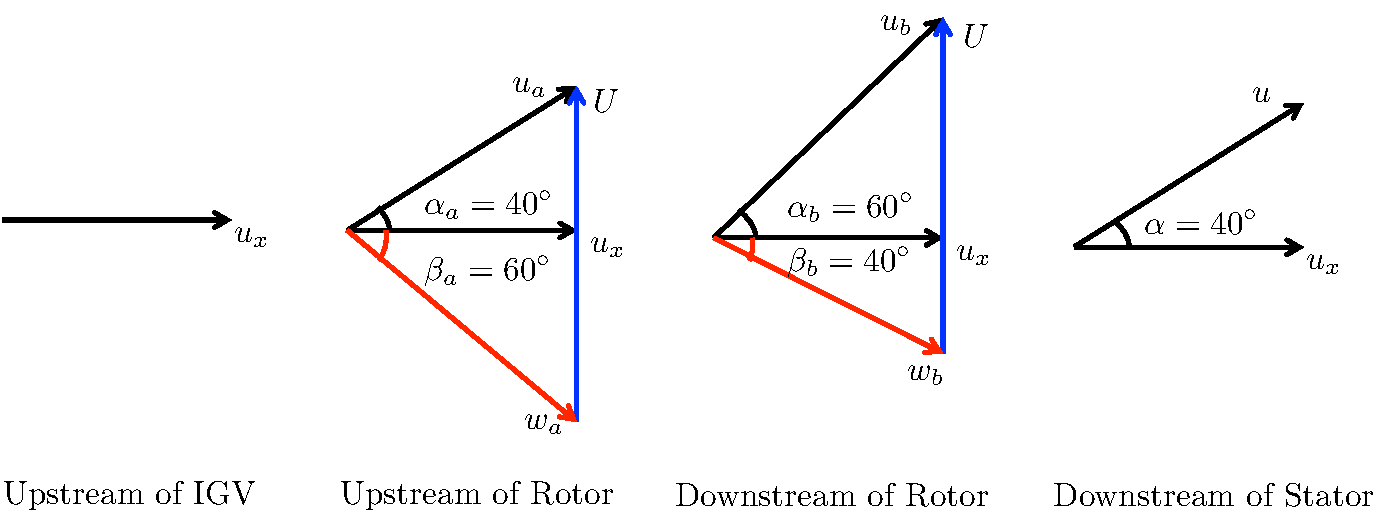
\includegraphics[width=160mm]{problem1b.pdf}
					\caption{\label{FIG_1B} Velocity triangles at four stations.}
				\end{center}
			\end{figure}
		\item (10 pts)
			The power required is given by
			\begin{equation}
				\begin{aligned}
					P_c &= \dot{m}_a(h_{0b}-h_{0a})\\
					&= \dot{m}_aU^2\left[1-\frac{u_x}{U}(\tan(\alpha_a)+\tan(\beta_b))\right] \ .
				\end{aligned}
			\end{equation}
			
			Furthermore, $\dot{m}_a=\rho u_x A$ and
			\begin{equation}
				\label{EQ_AREA}
				\begin{aligned}
					A &= \pi(r_\mathrm{tip}^2-r_\mathrm{hub}^2)\\
					&=\pi r_\mathrm{tip}^2\left[1-\left(\frac{r_\mathrm{hub}}{r_\mathrm{tip}}\right)^2\right]\\
					&=\pi r_m^2 \left(\frac{2}{1+\frac{r_\mathrm{hub}}{r_\mathrm{tip}}}\right)^2\left[1-\left(\frac{r_\mathrm{hub}}{r_\mathrm{tip}}\right)^2\right]\\
					&=0.125\ \mathrm{m^2}\ .
				\end{aligned}
			\end{equation}
			Since $\rho=1.2$ kg/m$^3$ for air at 20$^\circ$ and 1 atm and $u_x=125$ m/s, $\dot{m}_a=18.8$ kg/s. 
			
			Additionally,  $U=ux(\tan(\alpha_a)+\tan(\beta_a))=321$ m/s. Therefore, $\boxed{P=680\ \mathrm{kW}}$. 
			
			The rotational speed is $N=U/(2\pi r_m)=\boxed{170\ \mathrm{RPS}}	$ or $\boxed{10,200\ \mathrm{RPM}}$	
		\end{enumerate}
%%%%%%%%%%%%%%%%%%%%%%%%%%%%%%%%%%%%%%%%%%%%%%%%%%%%%%%%%%%%%%%%%%%%%%%%%%%%%%%%  
\section{Problem 2: Compressor Map (40 pts)}
\begin{enumerate}[label=(\alph*)]
	\item (10 pts)
		Firstly, the turbine inlet temperature is given to be $\boxed{T_{04}=1600\ \mathrm{K}}$. The mass flow of air through the compressor is given by 
		\begin{equation}				
			\begin{aligned}
				\dot m_c&=\frac{T}{(U_e-U_0)+\beta(U_{1e}-U_0)}\ ,
			\end{aligned}
		\end{equation}
		where the thrust is known to be $T=3400$ N and the bypass ratio is $\beta=2.9$. Additionally, $U_0=M_0a_0=$ m/s at 30 kft. 
		
		$U_e$ and $U_{e1}$ are found in a manner similar to the real turbofan case in the first problem set (details are given in the solution code). The primary difference is the use of the stage efficiency, $\eta_{st}$. For Point A, the reference condition is taken to be the design condition (i.e., engine operation at 30 kft.). Hence, $\boxed{\eta_{st}=0.87}$. 
		
		Furthermore, the stagnation pressure leaving the compressor is $\boxed{p_{03}=4.3\ \mathrm{bar}}$ and the mass flow rate is $\boxed{\dot m_c=2.9\ \mathrm{kg/s}}$.
		
		Finally, by inverting Eq.~\ref{EQ_AREA}, one can find $\bar{r}$ once $A$ is known since $r_\mathrm{hub}/r_\mathrm{tip}=0.6$. $A$ is found using relations for isentropic compressible flow (see code) with $M_{2.5}=u_{2.5}/a_{2.5}$ where $u_{2.5}=u_{x,\mathrm{ref}}=75\ \mathrm{m/s}$. Hence, $\boxed{\bar{r}=0.12\ \mathrm{m}}$. It should be noted that in actuality the mean radius may change to preserve the axial velocity through the compressor. Hence, $\bar{r}$ should be thought of as an effective mean radius.
	\item (10 pts)
		The mass flow is slightly less than that used in the previous analysis (about 3 kg/s at 30 kft); however, is within a somewhat reasonable range. The maximum diameter of the Honda Jet engine is 21.2 in. The tip radius was found to be 5.7 in. Hence, the compressor in this analysis is somewhat smaller than expected. Also, it should be noted that the compressor pressure ratio found is significantly less than the design condition ($\pi_c=5.2$ rather than $\pi_c=12$).
	\item (10 pts)
		The compressor efficiency, $\eta_c$ is given by
		\begin{equation}
			\label{EQ_ETAC}
			\eta_c=\frac{\pi_c^{\frac{\gamma-1}{\gamma}}-1}{\tau_c-1}
		\end{equation}
		Now, the temperature ratio is found by the update relation
		\begin{equation}
			\begin{aligned}
				T_{0,i+1} &= T_{0,i}+\frac{U\Delta u_\theta}{c_p}\\ \implies
				T_{03} &= T_{02.5}+n_\mathrm{stages}\frac{U\Delta u_\theta}{c_p} \\
				\implies \tau_c&=1+n_\mathrm{stages}\frac{U\Delta u_\theta}{c_pT_{02.5}}\ .
			\end{aligned}
		\end{equation}
		For a single stage, the update relation for pressure is given by 
		\begin{equation}
			\begin{aligned}
				p_{0,i+1} &= p_{0,i}\left(1+\eta_{st}\frac{U\Delta u_\theta}{c_pT_{0,i}}\right)^{\frac{\gamma}{\gamma-1}}\\ 
				&= p_{0,i}\left[1+\eta_{st}\frac{U\Delta u_\theta}{c_p\left(T_{02.5}+i\frac{U\Delta u_\theta}{c_p}\right)}\right]^{\frac{\gamma}{\gamma-1}}\\
				&=p_{0,i}\left[1+\eta_{st}\left(\frac{c_pT_{02.5}}{U\Delta u_\theta}+i\right)^{-1}\right]^{\frac{\gamma}{\gamma-1}}\\
				\implies \pi_c&=\left[\prod_{i=1}^{n_\mathrm{stages}} 1+\eta_{st}\left(\frac{c_pT_{02.5}}{U\Delta u_\theta}+i\right)^{-1}\right]^{\frac{\gamma}{\gamma-1}}
			\end{aligned}
		\end{equation}
		Substitution into Eq.~\ref{EQ_ETAC} yields
		\begin{equation}
			\eta_c=\boxed{\left[\prod_{i=1}^{n_\mathrm{stages}}1+\eta_{st}\left(\frac{c_pT_{02.5}}{U\Delta u_\theta}+i\right)^{-1}\right]-\left(n_\mathrm{stages}\frac{U\Delta u_\theta}{c_pT_{02.5}}\right)^{-1}}
		\end{equation}
	\item (10 pts)
		The compressor map is shown in Fig.~\ref{FIG_CM}. Your map may differ given your assumptions.		
		\begin{figure}[!ht!]
			\begin{center}
				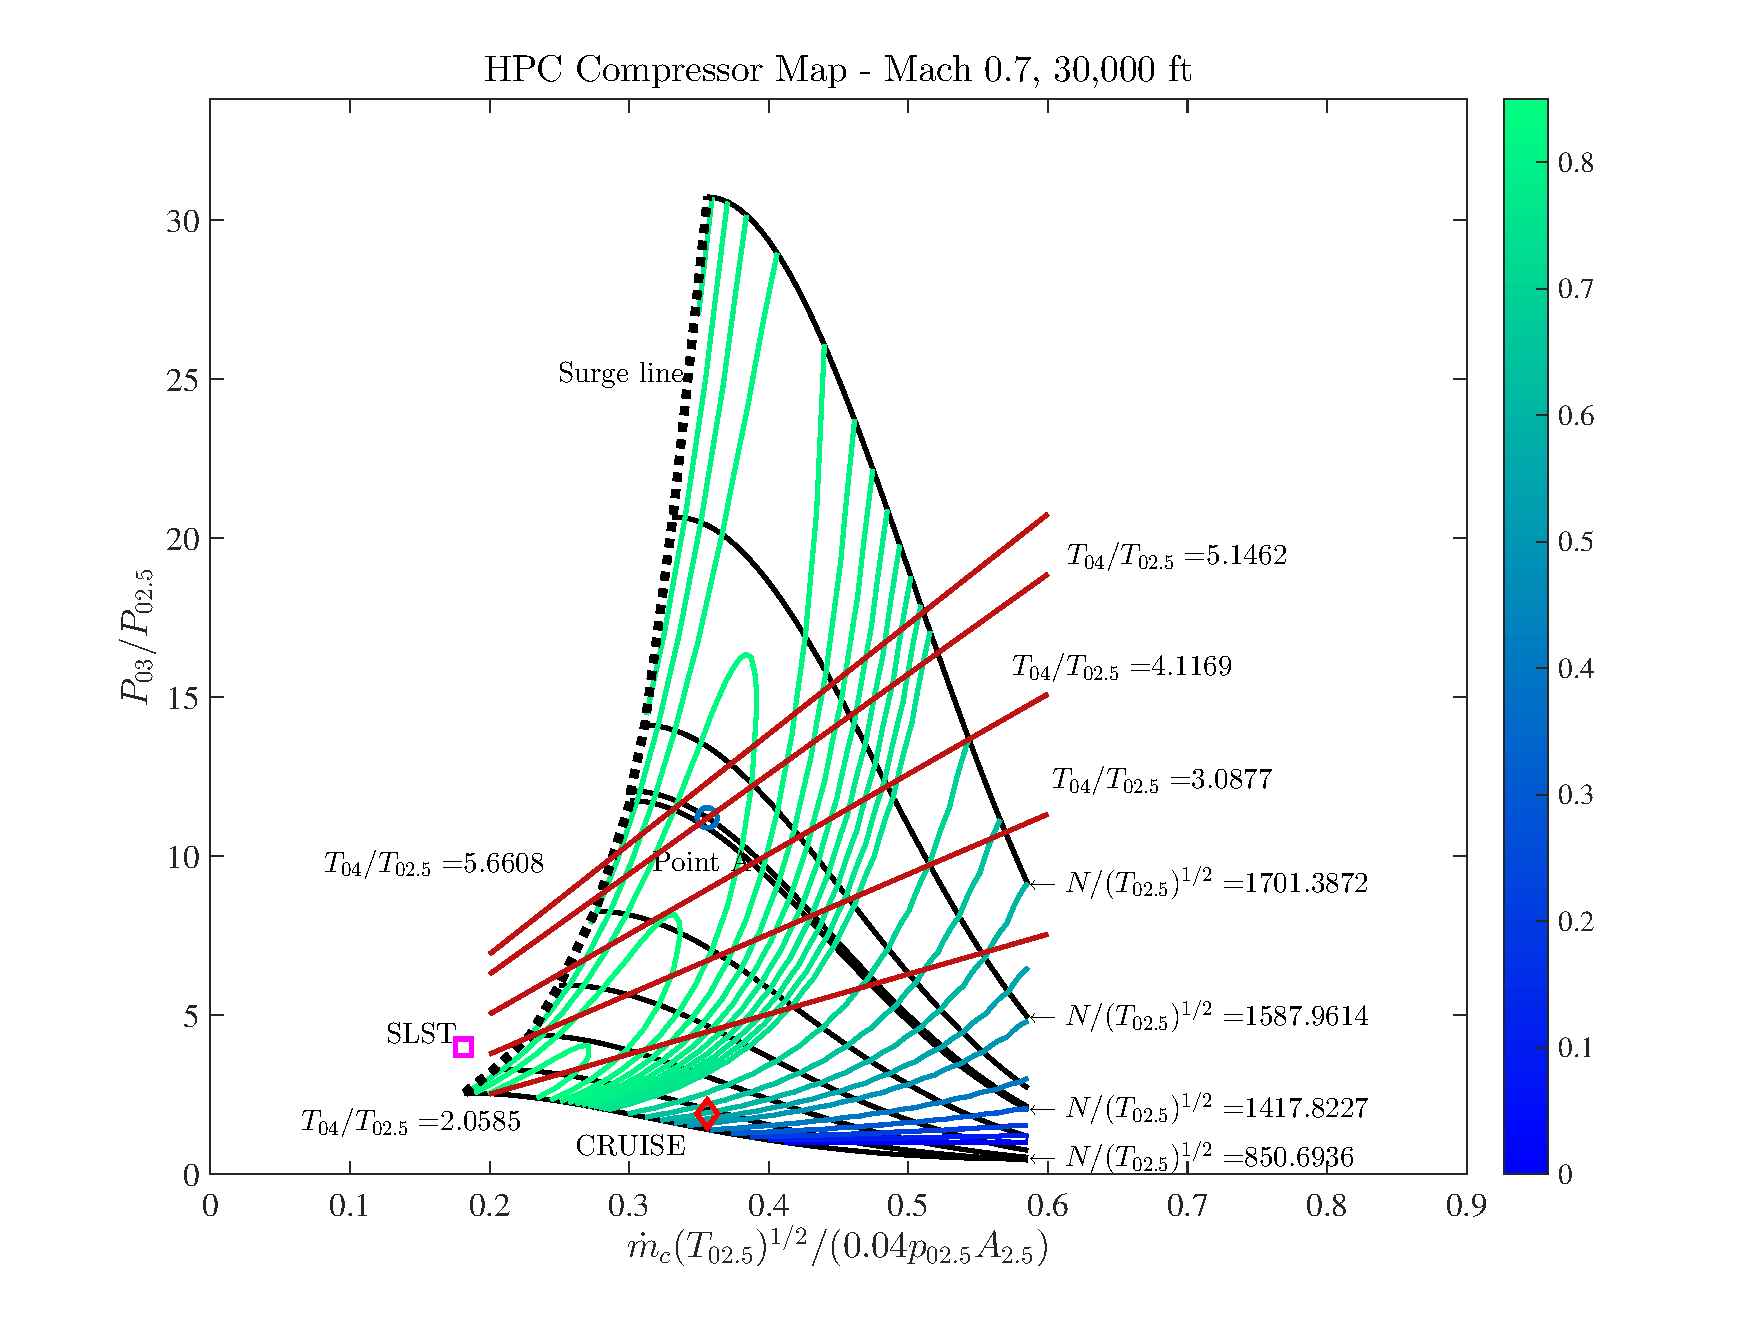
\includegraphics[width=180mm]{compressorMap.pdf}
				\caption{\label{FIG_CM} Compressor map. Red lines are of constant $T_{04}/T_{02.5}$, contour lines are of constant $\eta_c$, and black lines are of constant $N/T_{02.5}^{1/2}$.}
			\end{center}
		\end{figure}
\end{enumerate}
%%%%%%%%%%%%%%%%%%%%%%%%%%%%%%%%%%%%%%%%%%%%%%%%%%%%%%%%%%%%%%%%%%%%%%%%%%%%%%%%  
\section{Problem 3: Different Operating Conditions (30 pts)}		
\begin{enumerate}[label=(\alph*)]
	\item (10 pts)
		The CRUISE point is marked in Fig.~\ref{FIG_CM} with a red diamond.
	\item (10 pts)
		A drag calculation for this point is not required since it is negligible; thrust is primarily used in this stage to accelerate the aircraft and to climb. 
		
		The sea-level static thrust is marked on the graph with a magenta square. It is shown that this is not an operable condition in our analysis.
	\item (10 pts)
		This analysis shows that the current compressor design is not operable during takeoff. This differs from the cruise condition, which is simply inefficient.
\end{enumerate}
%%%%%%%%%%%%%%%%%%%%%%%%%%%%%%%%%%%%%%%%%%%%%%%%%%%%%%%%%%%%%%%%%%%%%%%%%%%%%%%%  	
\end{document}